%auto-ignore
\section{Experiments}
\label{sec:results}

Having detailed how to specify and optimize guide programs in our system, in this section, we experimentally evaluate how well programs written in our system can learn generative models and approximate posterior samplers. Unless stated otherwise, we use the following settings for the experiments in this section:
%%%
\begin{itemize}
\item{The Adam optimization method~\cite{Adam} with $\alpha = 0.1$, $\beta_1 = 0.9$, and $\beta_2 = 0.99$.}
\item{One sample from $\guide$ per optimization step to estimate the expectation in Equation~\ref{eq:finalEstimator}.}
\end{itemize}

\subsection{Gaussian Mixture Model}
\label{sec:results_gmm}

We first consider the simple Gaussian mixture model program from Figure~\ref{fig:bn_oneLatent} Bottom. This program samples discrete random choices, so its gradient estimator will include an LR term. Alternatively, we could re-write the program slightly to explicitly marginalize out the discrete random choices; see Appendix~\ref{sec:appendix_code:gmmSumOut}. The gradient estimator for this program then reduces to the PW estimator, which will have lower variance. Lower variance comes at the cost of amortized inference, however, as this version of the program does not have a guide which can predict the latent cluster assignment given an observed point. We also consider a non-amortized, mean field version of the program for comparison.

Figure~\ref{fig:gmmResults} illustrates the performance of these programs after training for 200 steps on a synthetic datset of 100 points. We learn model parameters using regularized maximum likelihood estimation. On the left, we show how the ELBo changes during optimizaton. Even on a simple model such as this one, the ability to use the pure PW estimator leads to faster convergence and a better final objective score.
On the right, we show the estimated negative log likelihood of a separate synthetic test set under each program after optimization. Here, we also include the tue model (i.e. the model used to synthesize the test/training data) for comparsion.
As suggested by its optimization performance, the model with discrete choices marginalized out performs best.
Note that the amortized guide program slightly out-performs the mean field guide program, indicating that the generalization provided by amortization has benefits for training generative models, in addition to enabling fast predictions of latent variables for previously-unseen observations.

\begin{figure}[!ht]
\begin{minipage}{0.5\linewidth}
\centering
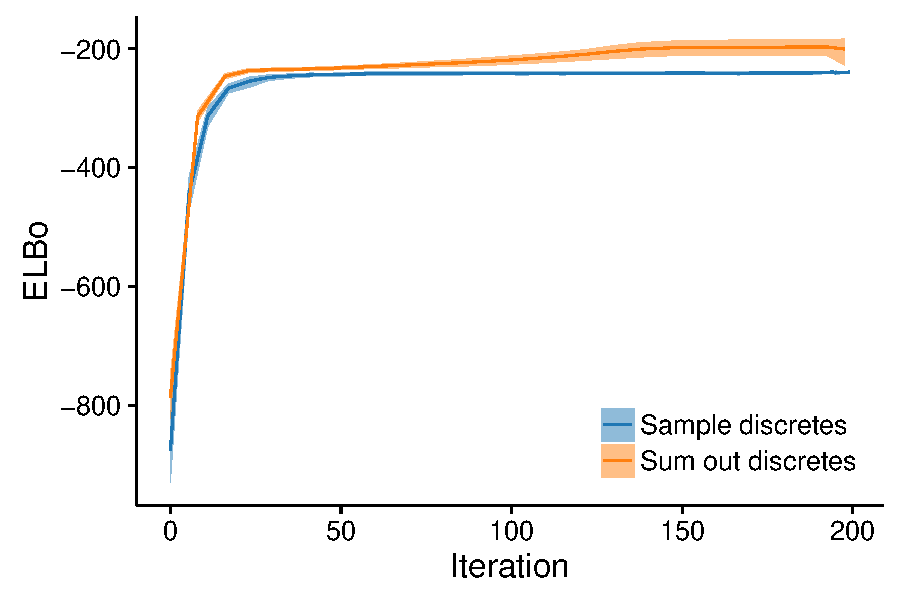
\includegraphics[width=\linewidth]{figs/results/gmm/elboProgress.pdf}
\end{minipage}
%
\begin{minipage}{0.5\linewidth}
\centering
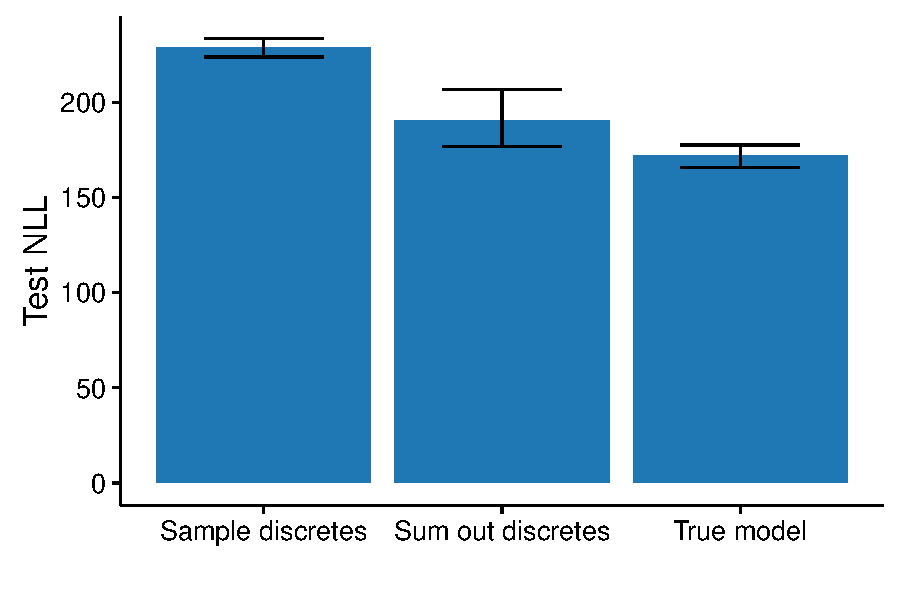
\includegraphics[width=\linewidth]{figs/results/gmm/nll.pdf}
\end{minipage}
\caption{Performance of simple Gaussian mixture model program. \emph{(Left)} ELBo optimization progress during training. \emph{(Right)} Negative log-likelihood of a held-out test set.}
\label{fig:gmmResults}
\end{figure}

% Other Bayes net examples??


\subsection{Variational Autoencoder}
\label{sec:results_vae}

Cite AEVB paper.

Show learned MNIST manifold?

Explore model uncertainty?

Explore mixture guides?

Consider factorial version (ie multiple latents)?


\subsection{Sigmoid Belief Network}
\label{sec:results_sbn}

Cite similarities between this model and the NVIL one.


\subsection{Latent Dirichlet Allocation}
\label{sec:results_lda}

Introduce the CoCoLab abstracts dataset (is there a citation for this yet?)

Just (manually-specified) mean-field guides, for now.

Show Top N words for each learned topic?


Things to try if we have time:
\begin{itemize}
\item{Simple bayesian NN (show how easy it is to do full variational Bayes)}
\item{HMM-type families: Deep kalman filter? Or other RNN VAE type thing?}
\item{PCFG (prob won’t work, but useful to understand). Continuous feature-passing version?}
\end{itemize}

